% Options for packages loaded elsewhere
\PassOptionsToPackage{unicode}{hyperref}
\PassOptionsToPackage{hyphens}{url}
\PassOptionsToPackage{dvipsnames,svgnames,x11names}{xcolor}
%
\documentclass[
  letterpaper,
  DIV=11,
  numbers=noendperiod]{scrartcl}

\usepackage{amsmath,amssymb}
\usepackage{iftex}
\ifPDFTeX
  \usepackage[T1]{fontenc}
  \usepackage[utf8]{inputenc}
  \usepackage{textcomp} % provide euro and other symbols
\else % if luatex or xetex
  \usepackage{unicode-math}
  \defaultfontfeatures{Scale=MatchLowercase}
  \defaultfontfeatures[\rmfamily]{Ligatures=TeX,Scale=1}
\fi
\usepackage{lmodern}
\ifPDFTeX\else  
    % xetex/luatex font selection
\fi
% Use upquote if available, for straight quotes in verbatim environments
\IfFileExists{upquote.sty}{\usepackage{upquote}}{}
\IfFileExists{microtype.sty}{% use microtype if available
  \usepackage[]{microtype}
  \UseMicrotypeSet[protrusion]{basicmath} % disable protrusion for tt fonts
}{}
\makeatletter
\@ifundefined{KOMAClassName}{% if non-KOMA class
  \IfFileExists{parskip.sty}{%
    \usepackage{parskip}
  }{% else
    \setlength{\parindent}{0pt}
    \setlength{\parskip}{6pt plus 2pt minus 1pt}}
}{% if KOMA class
  \KOMAoptions{parskip=half}}
\makeatother
\usepackage{xcolor}
\setlength{\emergencystretch}{3em} % prevent overfull lines
\setcounter{secnumdepth}{4}
% Make \paragraph and \subparagraph free-standing
\makeatletter
\ifx\paragraph\undefined\else
  \let\oldparagraph\paragraph
  \renewcommand{\paragraph}{
    \@ifstar
      \xxxParagraphStar
      \xxxParagraphNoStar
  }
  \newcommand{\xxxParagraphStar}[1]{\oldparagraph*{#1}\mbox{}}
  \newcommand{\xxxParagraphNoStar}[1]{\oldparagraph{#1}\mbox{}}
\fi
\ifx\subparagraph\undefined\else
  \let\oldsubparagraph\subparagraph
  \renewcommand{\subparagraph}{
    \@ifstar
      \xxxSubParagraphStar
      \xxxSubParagraphNoStar
  }
  \newcommand{\xxxSubParagraphStar}[1]{\oldsubparagraph*{#1}\mbox{}}
  \newcommand{\xxxSubParagraphNoStar}[1]{\oldsubparagraph{#1}\mbox{}}
\fi
\makeatother

\usepackage{color}
\usepackage{fancyvrb}
\newcommand{\VerbBar}{|}
\newcommand{\VERB}{\Verb[commandchars=\\\{\}]}
\DefineVerbatimEnvironment{Highlighting}{Verbatim}{commandchars=\\\{\}}
% Add ',fontsize=\small' for more characters per line
\newenvironment{Shaded}{}{}
\newcommand{\AlertTok}[1]{\textcolor[rgb]{0.58,0.85,0.30}{\textbf{\colorbox[rgb]{0.30,0.12,0.14}{#1}}}}
\newcommand{\AnnotationTok}[1]{\textcolor[rgb]{0.31,0.63,0.31}{#1}}
\newcommand{\AttributeTok}[1]{\textcolor[rgb]{0.65,0.15,0.64}{#1}}
\newcommand{\BaseNTok}[1]{\textcolor[rgb]{0.60,0.41,0.00}{#1}}
\newcommand{\BuiltInTok}[1]{\textcolor[rgb]{0.65,0.15,0.64}{#1}}
\newcommand{\CharTok}[1]{\textcolor[rgb]{0.31,0.63,0.31}{#1}}
\newcommand{\CommentTok}[1]{\textcolor[rgb]{0.63,0.63,0.65}{\textit{#1}}}
\newcommand{\CommentVarTok}[1]{\textcolor[rgb]{0.89,0.34,0.29}{\textit{#1}}}
\newcommand{\ConstantTok}[1]{\textcolor[rgb]{0.60,0.41,0.00}{#1}}
\newcommand{\ControlFlowTok}[1]{\textcolor[rgb]{0.65,0.15,0.64}{#1}}
\newcommand{\DataTypeTok}[1]{\textcolor[rgb]{0.65,0.15,0.64}{#1}}
\newcommand{\DecValTok}[1]{\textcolor[rgb]{0.60,0.41,0.00}{#1}}
\newcommand{\DocumentationTok}[1]{\textcolor[rgb]{0.89,0.34,0.29}{#1}}
\newcommand{\ErrorTok}[1]{\textcolor[rgb]{0.96,0.28,0.28}{\underline{#1}}}
\newcommand{\ExtensionTok}[1]{\textcolor[rgb]{0.25,0.47,0.95}{\textbf{#1}}}
\newcommand{\FloatTok}[1]{\textcolor[rgb]{0.60,0.41,0.00}{#1}}
\newcommand{\FunctionTok}[1]{\textcolor[rgb]{0.25,0.47,0.95}{#1}}
\newcommand{\ImportTok}[1]{\textcolor[rgb]{0.31,0.63,0.31}{#1}}
\newcommand{\InformationTok}[1]{\textcolor[rgb]{0.77,0.36,0.00}{#1}}
\newcommand{\KeywordTok}[1]{\textcolor[rgb]{0.65,0.15,0.64}{#1}}
\newcommand{\NormalTok}[1]{\textcolor[rgb]{0.22,0.23,0.26}{#1}}
\newcommand{\OperatorTok}[1]{\textcolor[rgb]{0.65,0.15,0.64}{#1}}
\newcommand{\OtherTok}[1]{\textcolor[rgb]{0.15,0.68,0.38}{#1}}
\newcommand{\PreprocessorTok}[1]{\textcolor[rgb]{0.65,0.15,0.64}{#1}}
\newcommand{\RegionMarkerTok}[1]{\textcolor[rgb]{0.16,0.50,0.73}{\colorbox[rgb]{0.08,0.19,0.26}{#1}}}
\newcommand{\SpecialCharTok}[1]{\textcolor[rgb]{0.00,0.52,0.74}{#1}}
\newcommand{\SpecialStringTok}[1]{\textcolor[rgb]{0.85,0.27,0.33}{#1}}
\newcommand{\StringTok}[1]{\textcolor[rgb]{0.31,0.63,0.31}{#1}}
\newcommand{\VariableTok}[1]{\textcolor[rgb]{0.89,0.34,0.29}{#1}}
\newcommand{\VerbatimStringTok}[1]{\textcolor[rgb]{0.85,0.27,0.33}{#1}}
\newcommand{\WarningTok}[1]{\textcolor[rgb]{0.85,0.27,0.33}{#1}}

\providecommand{\tightlist}{%
  \setlength{\itemsep}{0pt}\setlength{\parskip}{0pt}}\usepackage{longtable,booktabs,array}
\usepackage{calc} % for calculating minipage widths
% Correct order of tables after \paragraph or \subparagraph
\usepackage{etoolbox}
\makeatletter
\patchcmd\longtable{\par}{\if@noskipsec\mbox{}\fi\par}{}{}
\makeatother
% Allow footnotes in longtable head/foot
\IfFileExists{footnotehyper.sty}{\usepackage{footnotehyper}}{\usepackage{footnote}}
\makesavenoteenv{longtable}
\usepackage{graphicx}
\makeatletter
\def\maxwidth{\ifdim\Gin@nat@width>\linewidth\linewidth\else\Gin@nat@width\fi}
\def\maxheight{\ifdim\Gin@nat@height>\textheight\textheight\else\Gin@nat@height\fi}
\makeatother
% Scale images if necessary, so that they will not overflow the page
% margins by default, and it is still possible to overwrite the defaults
% using explicit options in \includegraphics[width, height, ...]{}
\setkeys{Gin}{width=\maxwidth,height=\maxheight,keepaspectratio}
% Set default figure placement to htbp
\makeatletter
\def\fps@figure{htbp}
\makeatother

\usepackage{setspace}
\usepackage[most]{tcolorbox}

\newtcolorbox{note}{
	colback=gray!10,
	colframe=gray!80!black,
	boxrule=0.5pt,
	arc=2mm,
	left=6pt,
	right=6pt,
	top=6pt,
	bottom=6pt,
	enhanced,
	before upper={\setstretch{1.2}},
}

\newtcolorbox{example}{
	colback=blue!10,
	colframe=blue!80!black,
	boxrule=0.5pt,
	arc=2mm,
	left=6pt,
	right=6pt,
	top=6pt,
	bottom=6pt,
	enhanced,
	before upper={\setstretch{1.2}},
}

% \usepackage[most]{tcolorbox}
% \newtcolorbox{shadednote}{
%   colback=gray!10,
%   colframe=gray!80!black,
%   boxrule=0.5pt,
%   arc=2mm,
%   left=6pt,
%   right=6pt,
%   top=6pt,
%   bottom=6pt,
%   enhanced,
%   before upper=\relax, % Do nothing, let it inherit
% }
% \newtcolorbox{shadednote}{
%   colback=gray!10,
%   colframe=gray!80!black,
%   boxrule=0.5pt,
%   arc=2mm,
%   left=6pt,
%   right=6pt,
%   top=6pt,
%   bottom=6pt,
% }
\usepackage{booktabs}
\usepackage{longtable}
\usepackage{array}
\usepackage{multirow}
\usepackage{wrapfig}
\usepackage{float}
\usepackage{colortbl}
\usepackage{pdflscape}
\usepackage{tabu}
\usepackage{threeparttable}
\usepackage{threeparttablex}
\usepackage[normalem]{ulem}
\usepackage{makecell}
\usepackage{xcolor}
\KOMAoption{captions}{tableheading}
\makeatletter
\@ifpackageloaded{caption}{}{\usepackage{caption}}
\AtBeginDocument{%
\ifdefined\contentsname
  \renewcommand*\contentsname{Table of contents}
\else
  \newcommand\contentsname{Table of contents}
\fi
\ifdefined\listfigurename
  \renewcommand*\listfigurename{List of Figures}
\else
  \newcommand\listfigurename{List of Figures}
\fi
\ifdefined\listtablename
  \renewcommand*\listtablename{List of Tables}
\else
  \newcommand\listtablename{List of Tables}
\fi
\ifdefined\figurename
  \renewcommand*\figurename{Figure}
\else
  \newcommand\figurename{Figure}
\fi
\ifdefined\tablename
  \renewcommand*\tablename{Table}
\else
  \newcommand\tablename{Table}
\fi
}
\@ifpackageloaded{float}{}{\usepackage{float}}
\floatstyle{ruled}
\@ifundefined{c@chapter}{\newfloat{codelisting}{h}{lop}}{\newfloat{codelisting}{h}{lop}[chapter]}
\floatname{codelisting}{Listing}
\newcommand*\listoflistings{\listof{codelisting}{List of Listings}}
\makeatother
\makeatletter
\makeatother
\makeatletter
\@ifpackageloaded{caption}{}{\usepackage{caption}}
\@ifpackageloaded{subcaption}{}{\usepackage{subcaption}}
\makeatother
\makeatletter
\@ifpackageloaded{tcolorbox}{}{\usepackage[skins,breakable]{tcolorbox}}
\makeatother
\makeatletter
\@ifundefined{shadecolor}{\definecolor{shadecolor}{named}{white}}{}
\makeatother
\makeatletter
\@ifundefined{codebgcolor}{\definecolor{codebgcolor}{HTML}{f8f8f8}}{}
\makeatother
\makeatletter
\ifdefined\Shaded\renewenvironment{Shaded}{\begin{tcolorbox}[frame hidden, colback={codebgcolor}, sharp corners, borderline west={3pt}{0pt}{shadecolor}, breakable, enhanced, boxrule=0pt]}{\end{tcolorbox}}\fi
\makeatother

\ifLuaTeX
  \usepackage{selnolig}  % disable illegal ligatures
\fi
\usepackage{bookmark}

\IfFileExists{xurl.sty}{\usepackage{xurl}}{} % add URL line breaks if available
\urlstyle{same} % disable monospaced font for URLs
\hypersetup{
  pdftitle={Transform Your Terminal with Ghostty and Yazi},
  pdfauthor={Jake Jing},
  colorlinks=true,
  linkcolor={blue},
  filecolor={Maroon},
  citecolor={Blue},
  urlcolor={Blue},
  pdfcreator={LaTeX via pandoc}}


\title{Transform Your Terminal with Ghostty and Yazi}
\author{Jake Jing}
\date{July 18, 2025}

\begin{document}
\maketitle

\renewcommand*\contentsname{Contents}
{
\hypersetup{linkcolor=}
\setcounter{tocdepth}{4}
\tableofcontents
}
\listoffigures
\listoftables

\clearpage

\section{Introduction}\label{introduction}

Why I Switched from Kitty and Vifm to Ghostty and Yazi? After years of
experimenting with different terminal emulators and file managers, I've
finally found my favorite combination: Ghostty and Yazi. These have
recently gained a lot of popularity in the community. Briefly put,
\href{https://github.com/ghostty-org/ghostty}{Ghostty} is a modern
terminal emulator that is fast, feature-rich, and native.
\href{https://github.com/sxyazi/yazi}{Yazi} is a blazing-fast terminal
file manager. Together, they have transformed my daily workflow. In this
blog, I'll show you how to set them up on your own computer, so you can
supercharge your terminal experience just like I did.

Note: here I assume the default fish shell is used. You can install it
in \href{https://medium.com/p/6f9610276c33}{this blog}.

\section{Install Ghostty}\label{install-ghostty}

\subsection{brew install ghostty}\label{brew-install-ghostty}

\begin{Shaded}
\begin{Highlighting}[]
\ExtensionTok{brew}\NormalTok{ install }\AttributeTok{{-}{-}cask}\NormalTok{ ghostty}
\end{Highlighting}
\end{Shaded}

\subsection{set ghostty as default terminal emulator on
mac}\label{set-ghostty-as-default-terminal-emulator-on-mac}

\begin{itemize}
\tightlist
\item
  \begin{enumerate}
  \def\labelenumi{(\arabic{enumi})}
  \tightlist
  \item
    Install the ``RCDefaultApp.prefPane'' plugin
  \end{enumerate}
\end{itemize}

This plugin is used to set the default app for opening terminal in your
system.

\begin{Shaded}
\begin{Highlighting}[]
\FunctionTok{git}\NormalTok{ clone https://github.com/JakeJing/fishconfig.git}
\FunctionTok{sudo}\NormalTok{ mv fishconfig/kitty/RCDefaultApp.prefPane /Library/PreferencePanes/}
\end{Highlighting}
\end{Shaded}

\begin{itemize}
\tightlist
\item
  \begin{enumerate}
  \def\labelenumi{(\arabic{enumi})}
  \setcounter{enumi}{1}
  \tightlist
  \item
    Set ghostty as the ``default app'' for opening terminal
  \end{enumerate}
\end{itemize}

Go to system preferences -\textgreater{} default Apps -\textgreater{}
click the ``default Apps'' -\textgreater{} URLS -\textgreater{}
x-man-page -\textgreater{} set the default application as ``ghostty''.

\begin{figure}[H]

{\centering 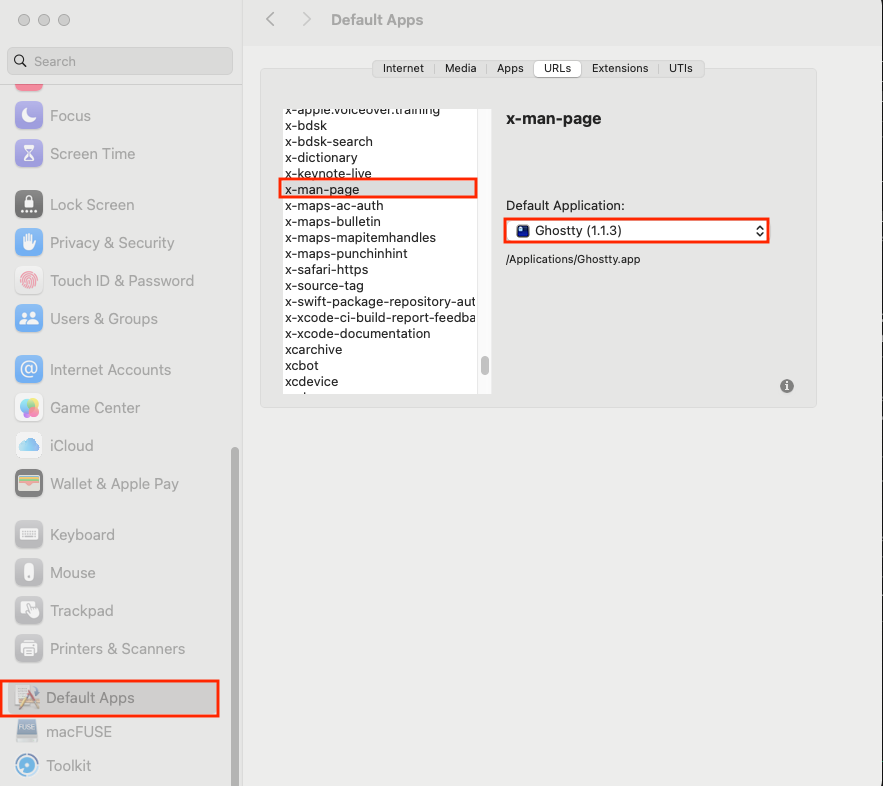
\includegraphics{./images/ghostty-default.png}

}

\caption{Set ghostty as default app for opening terminal}

\end{figure}%

\begin{itemize}
\tightlist
\item
  \begin{enumerate}
  \def\labelenumi{(\arabic{enumi})}
  \setcounter{enumi}{2}
  \tightlist
  \item
    Add keyboard shortcut (shift-cmd-1) to open a new Ghostty window
    here
  \end{enumerate}
\end{itemize}

You can set a keyboard shortcut to open Ghostty here. However, the
default option only works when your cursor is on a folder. To enable it
when your cursor is on a file, you can create a new service using the
Automator application. To do this, go to Automator -\textgreater{} Quick
Action, and follow the steps in the image below.

\begin{figure}[H]

{\centering 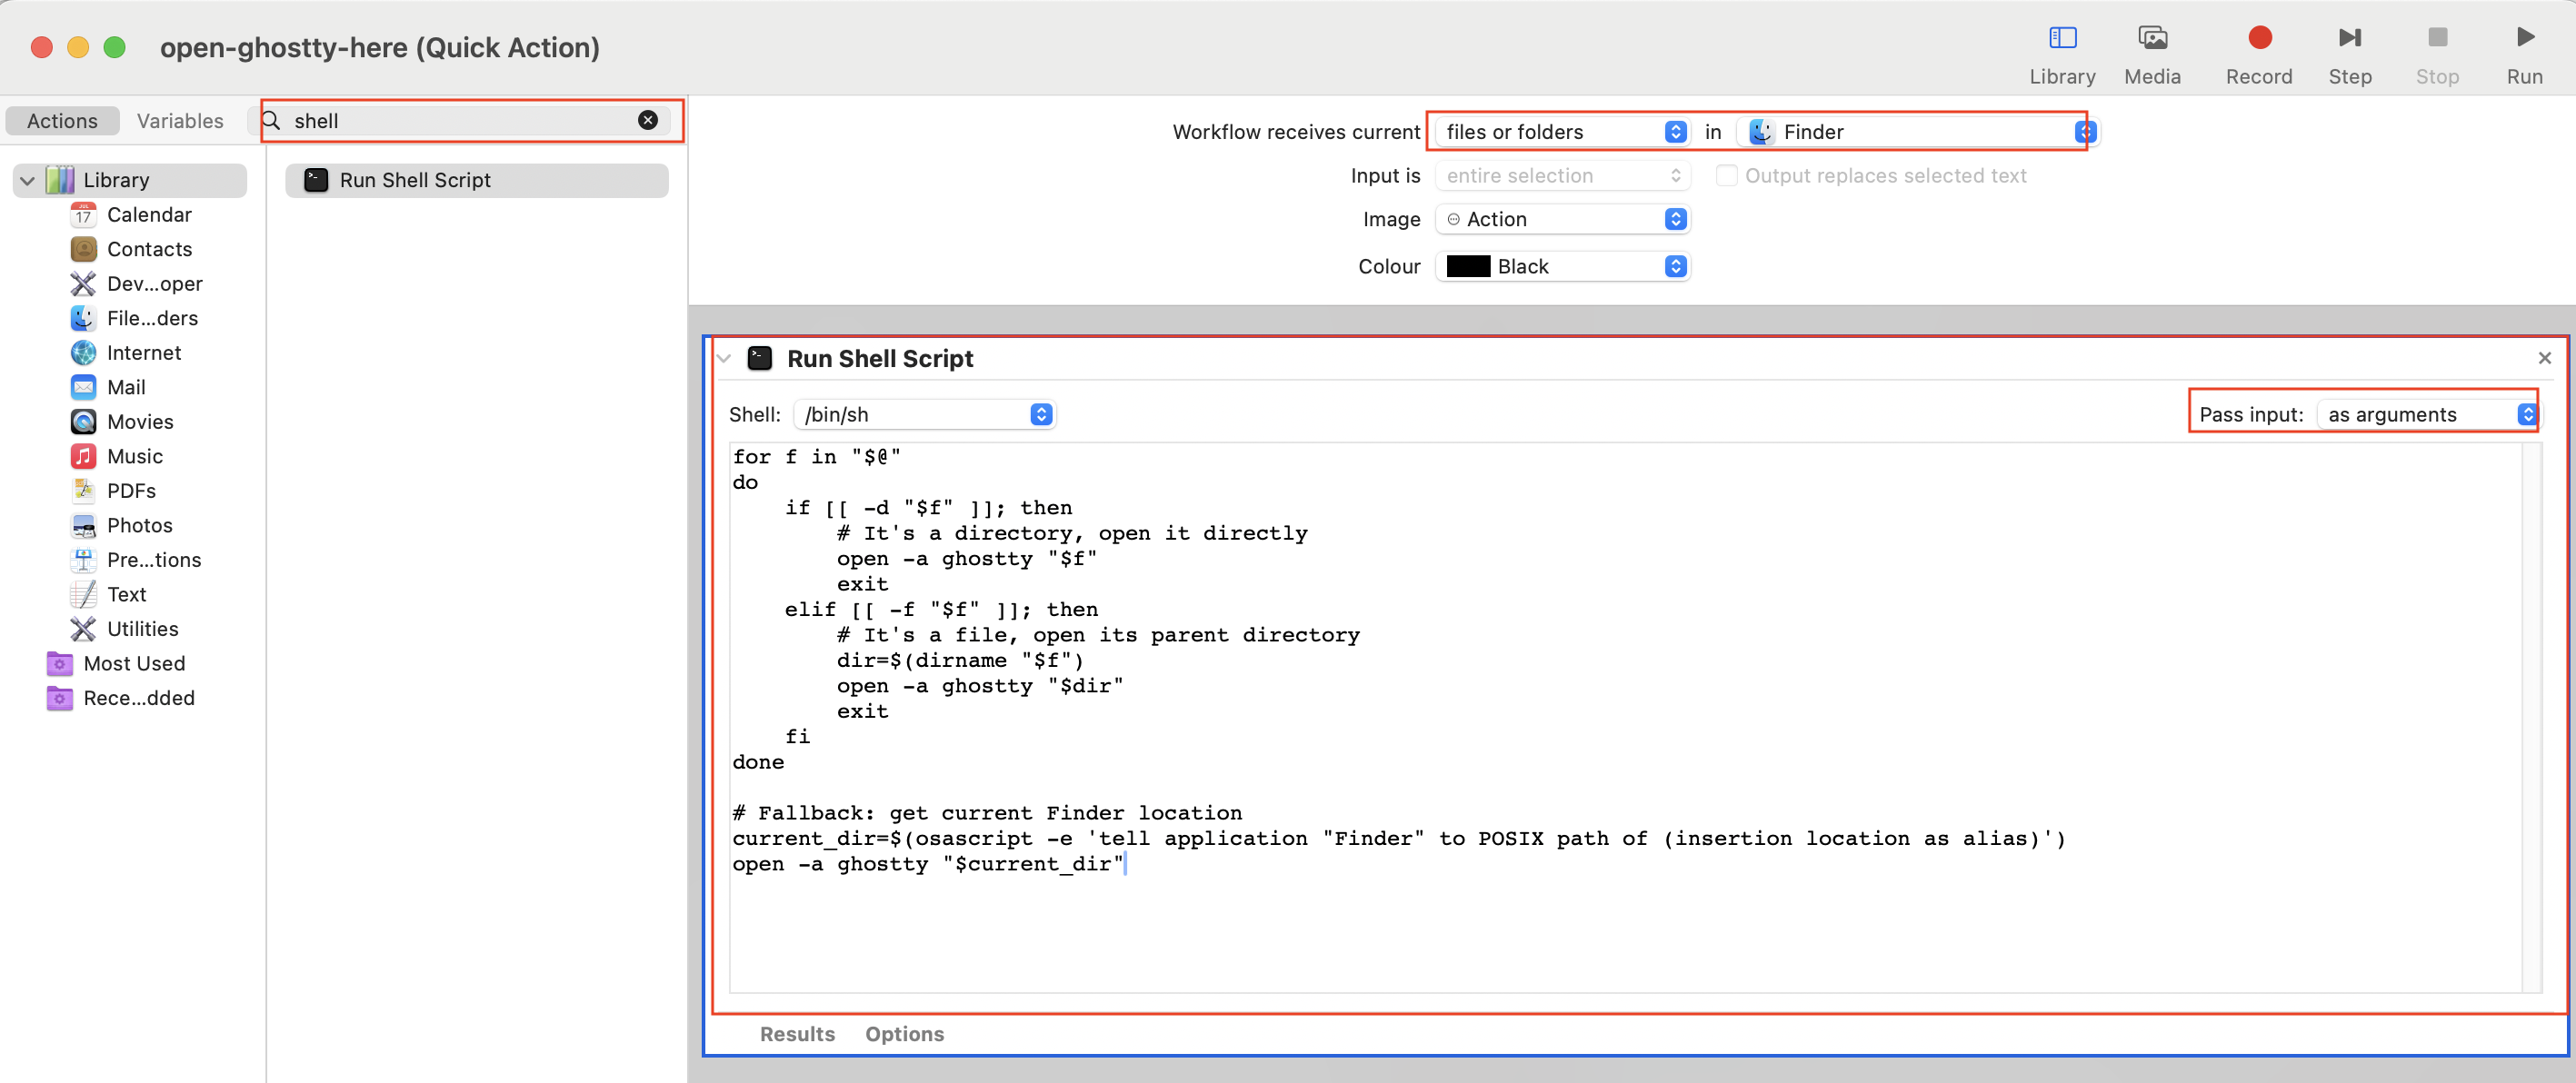
\includegraphics{./images/automator-quick-action.png}

}

\caption{Automator Quick Action}

\end{figure}%

After that, you can go to System Preferences -\textgreater{} Keyboard
-\textgreater{} Shortcuts -\textgreater{} Services -\textgreater{}
open-ghostty-here to add it (shift-cmd-1).

\begin{figure}[H]

{\centering 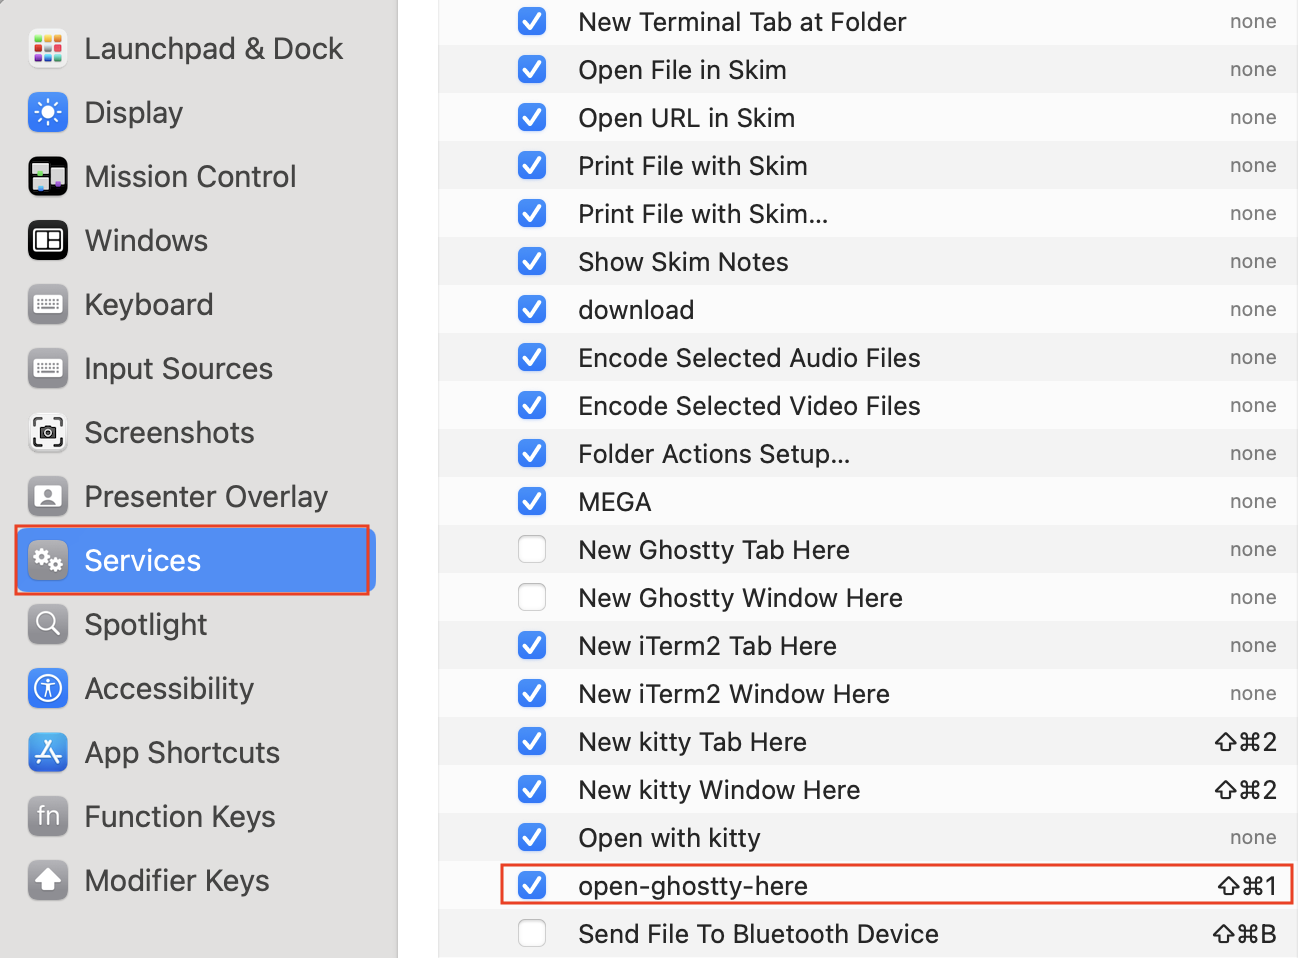
\includegraphics{./images/ghostty-window-here.png}

}

\caption{Add keyboard shortcut to open Ghostty here}

\end{figure}%

This will automatically open a new Ghostty window here when you press
shift-cmd-1. If there is an ongoing Ghostty window, it will open a new
tab instead. So far there is no easy way to always open a new window
(rather than a new tab or a new process) on mac, as far as I know.

\begin{Shaded}
\begin{Highlighting}[]
\CommentTok{\# check the services}
\FunctionTok{ls}\NormalTok{ \textasciitilde{}/Library/Services/}
\end{Highlighting}
\end{Shaded}

\begin{itemize}
\tightlist
\item
  \begin{enumerate}
  \def\labelenumi{(\arabic{enumi})}
  \setcounter{enumi}{3}
  \tightlist
  \item
    add configuration file for ghostty
  \end{enumerate}
\end{itemize}

\begin{Shaded}
\begin{Highlighting}[]
\FunctionTok{wget}\NormalTok{ https://raw.githubusercontent.com/JakeJing/dotfiles/refs/heads/main/.config/ghostty/config }\AttributeTok{{-}P}\NormalTok{ \textasciitilde{}/.config/ghostty/}
\end{Highlighting}
\end{Shaded}

\section{Install Yazi}\label{install-yazi}

\subsection{brew install yazi and its
dependencies}\label{brew-install-yazi-and-its-dependencies}

\begin{Shaded}
\begin{Highlighting}[]
\ExtensionTok{brew}\NormalTok{ update}
\ExtensionTok{brew}\NormalTok{ install yazi ffmpeg sevenzip jq poppler fd ripgrep fzf zoxide resvg imagemagick font{-}symbols{-}only{-}nerd{-}font}
\end{Highlighting}
\end{Shaded}

\subsection{set alias in fish config}\label{set-alias-in-fish-config}

\begin{Shaded}
\begin{Highlighting}[]
\CommentTok{\# yazi}
\BuiltInTok{alias}\NormalTok{ yz yazi}
\BuiltInTok{alias}\NormalTok{ y yazi}
\BuiltInTok{alias}\NormalTok{ a yazi}
\end{Highlighting}
\end{Shaded}

\subsection{add configuration file and keymap for
yazi}\label{add-configuration-file-and-keymap-for-yazi}

\begin{Shaded}
\begin{Highlighting}[]
\CommentTok{\# clone my dotfiles}
\FunctionTok{git}\NormalTok{ clone https://github.com/JakeJing/dotfiles.git}
\CommentTok{\# move yazi config}
\FunctionTok{mv}\NormalTok{ dotfiles/.config/yazi }\AttributeTok{{-}P}\NormalTok{ \textasciitilde{}/.config/yazi/}
\end{Highlighting}
\end{Shaded}

\begin{figure}[H]

{\centering 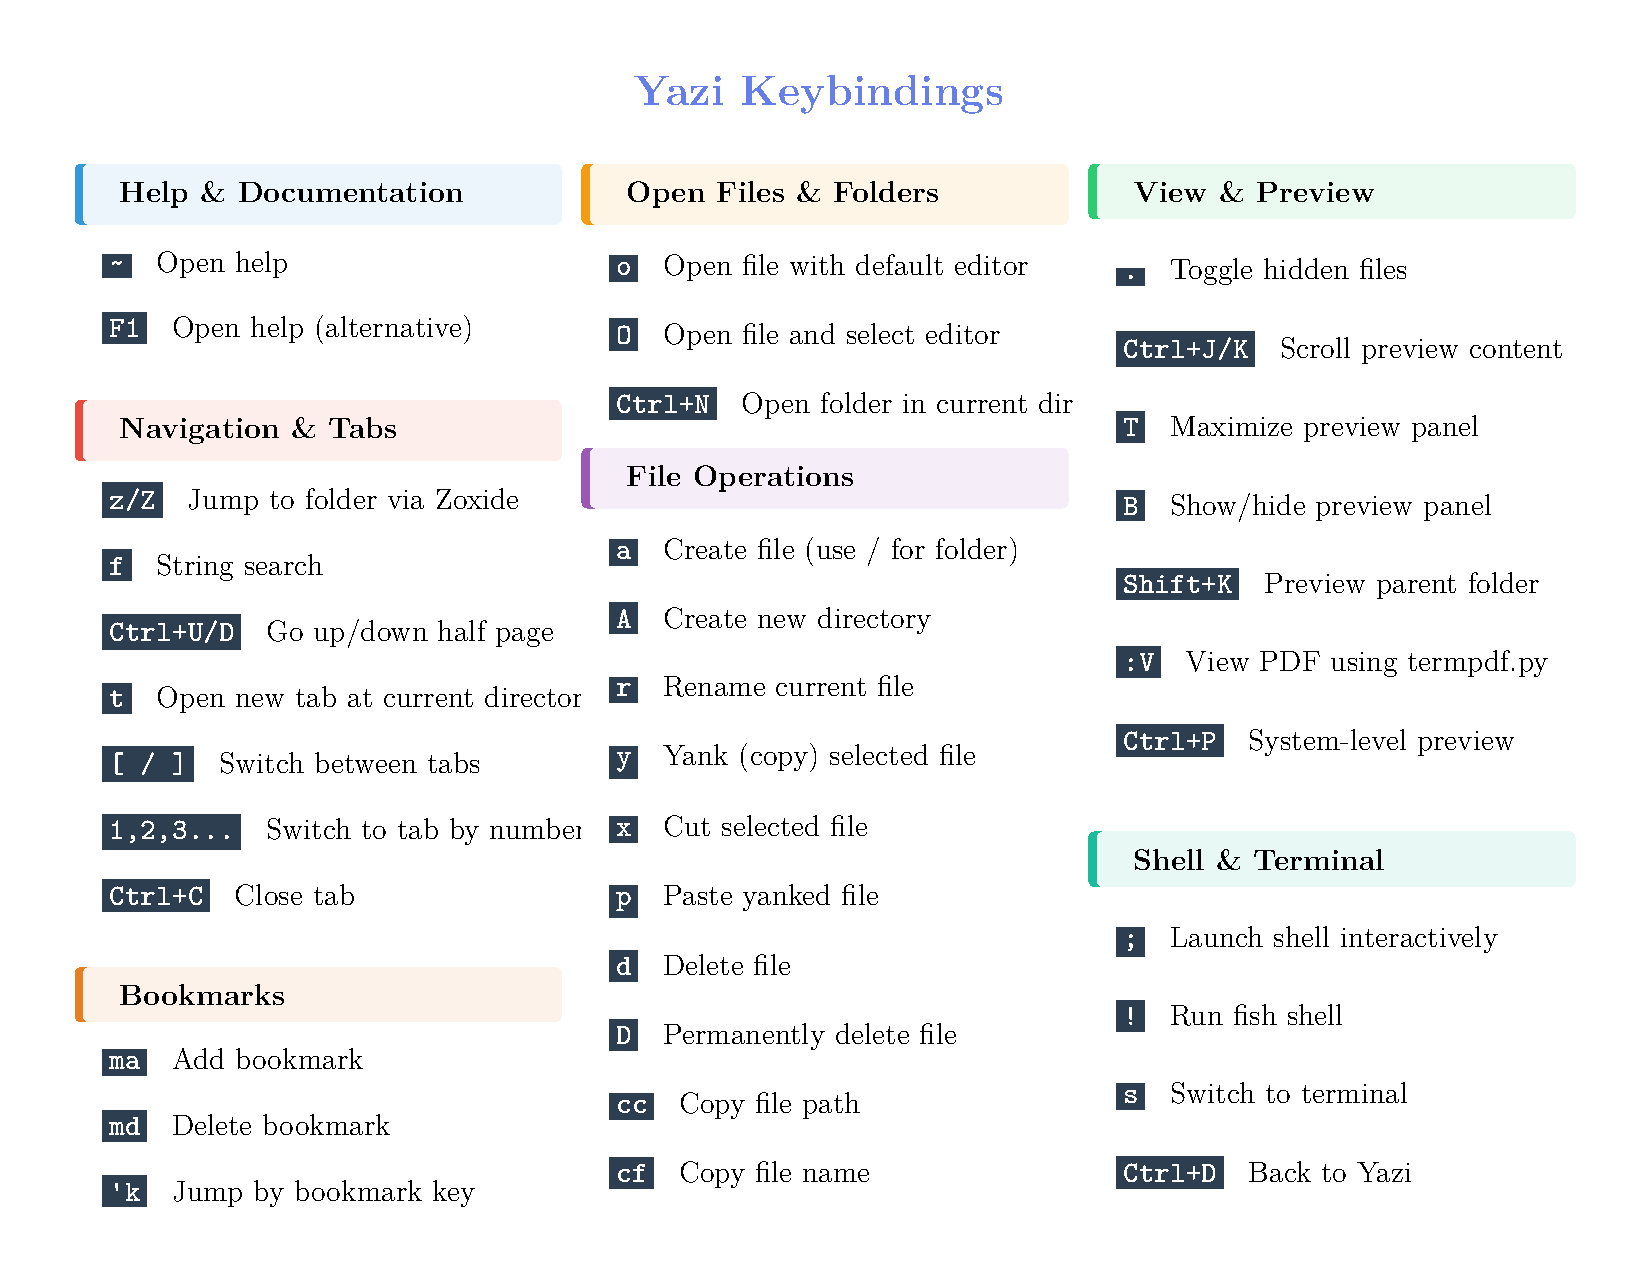
\includegraphics[width=1\textwidth,height=\textheight]{cheatsheet/yazi.pdf}

}

\caption{Useful Yazi Keybindings}

\end{figure}%




\end{document}
